%% Version 5.0, 2 January 2020
%
%%%%%%%%%%%%%%%%%%%%%%%%%%%%%%%%%%%%%%%%%%%%%%%%%%%%%%%%%%%%%%%%%%%%%%
% TemplateV5.tex --  LaTeX-based template for submissions to the 
% American Meteorological Society
%
%%%%%%%%%%%%%%%%%%%%%%%%%%%%%%%%%%%%%%%%%%%%%%%%%%%%%%%%%%%%%%%%%%%%%
% PREAMBLE
%%%%%%%%%%%%%%%%%%%%%%%%%%%%%%%%%%%%%%%%%%%%%%%%%%%%%%%%%%%%%%%%%%%%%

%% Start with one of the following:
% DOUBLE-SPACED VERSION FOR SUBMISSION TO THE AMS
\documentclass{ametsocV5}

% TWO-COLUMN JOURNAL PAGE LAYOUT---FOR AUTHOR USE ONLY
% \documentclass[twocol]{ametsocV5}


% Enter packages here. If too many math alphabets are used,
% remove unnecessary packages or define hmmax and bmmax as necessary.

%\newcommand{\hmmax}{0}
%\newcommand{\bmmax}{0}
\usepackage{amsmath,amsfonts,amssymb,bm}
\usepackage{mathptmx}%{times}
\usepackage{newtxtext}
\usepackage{newtxmath}
\usepackage{natbib}


%%%%%%%%%%%%%%%%%%%%%%%%%%%%%%%%

%%% To be entered by author:

%% May use \\ to break lines in title:

\title{Quantifying Uncertainty in Forecast-Based Anticipatory Action Triggers Using Bootstrapping Methods}

%%% Enter authors' names, as you see in this example:
%%% Use \correspondingauthor{} and \thanks{Current Affiliation:...}
%%% immediately following the appropriate author.
%%%
%%% Note that the \correspondingauthor{} command is NECESSARY.
%%% The \thanks{} commands are OPTIONAL.

    %\authors{Author One\correspondingauthor{Author name, email address}
% and Author Two\thanks{Current affiliation: American Meteorological Society, 
    % Boston, Massachusetts.}}

\author{%
Max Mauerman\affmark[1]\correspondingauthor{Max Mauerman, max.mauerman@columbia.edu}, Kevin Schwarzwald\affmark[1], Daniel Osgood\affmark[1], Nathan Lenssen\affmark[2], and Abdel-Lathif Younous\affmark[3]\\
\affaddr{\affmark[1] Columbia University Climate School}\\
\affaddr{\affmark[2] Colorado School of Mines \& NSF National Center for Atmospheric Research}\\
\affaddr{\affmark[3] United Nations World Food Programme}\\
}

%%%%%%%%%%%%%%%%%%%%%%%%%%%%%%%%%%%%%%%%%%%%%%%%%%%%%%%%%%%%%%%%%%%%%
% ABSTRACT
%
% Enter your abstract here
% Abstracts should not exceed 250 words in length!
%
 

\abstract{As of 2022, nearly 5 million smallholder farmers across a dozen countries are covered by Anticipatory Action (AA) programs \citep{chaves-gonzalez_anticipatory_2022}, which are aid schemes triggered if seasonal forecasts of rainfall cross a locally-determined threshold. AA thresholds are often calculated to meet a donor- or government-specified expected trigger frequency \citep{coughlan_de_perez_adapting_2022,world_food_programme_10_2024}. However, the observational rainfall record in many regions with AA programs is limited, and interannual and interdecadal autocorrelation in the climate patterns driving seasonal rainfall further reduce the effective sample size used to calculate these thresholds \citep{martinez_seasonal_2022}. Thus, AA triggers are highly sensitive to the limited observational record, increasing the risk that action is not triggered when it is needed or that programs become financially unsustainable due to excessive triggers. In practice, forecasters are aware of this uncertainty, and ad hoc decisions on whether to trigger action are often made if seasonal forecasts are close to the threshold. Seeking a more formalized, statistically sound alternative to ad hoc approaches, governments and humanitarian agencies have asked for transparent and intuitive metrics for forecast trigger uncertainty. To address this demand, we develop a method for quantifying the uncertainty in thresholds due to a limited observational record using bootstrap resampling. Examining United Nations operational AA forecasts in sub-Saharan Africa, we demonstrate how our method provides a better quantification of critical underlying uncertainty, enabling these AA systems to meet the state-of-the-art demanded by donors and the WMO.}
\begin{document}

%% Necessary!
\maketitle

%%%%%%%%%%%%%%%%%%%%%%%%%%%%%%%%%%%%%%%%%%%%%%%%%%%%%%%%%%%%%%%%%%%%%
% SIGNIFICANCE STATEMENT/CAPSULE SUMMARY
%%%%%%%%%%%%%%%%%%%%%%%%%%%%%%%%%%%%%%%%%%%%%%%%%%%%%%%%%%%%%%%%%%%%%
%
% If you are including an optional significance statement for a journal article or a required capsule summary for BAMS 
% (see www.ametsoc.org/ams/index.cfm/publications/authors/journal-and-bams-authors/formatting-and-manuscript-components for details), 
% please apply the necessary command as shown below:
%
% \statement
% Significance statement here.
%
% \capsule
% Capsule summary here.


%%%%%%%%%%%%%%%%%%%%%%%%%%%%%%%%%%%%%%%%%%%%%%%%%%%%%%%%%%%%%%%%%%%%%
% MAIN BODY OF PAPER
%%%%%%%%%%%%%%%%%%%%%%%%%%%%%%%%%%%%%%%%%%%%%%%%%%%%%%%%%%%%%%%%%%%%%
%

%% In all cases, if there is only one entry of this type within
%% the higher level heading, use the star form: 
%%
% \section{Section title}
% \subsection*{subsection}
% text...
% \section{Section title}

%vs

% \section{Section title}
% \subsection{subsection one}
% text...
% \subsection{subsection two}
% \section{Section title}

%%%
% \section{First primary heading}

% \subsection{First secondary heading}

% \subsubsection{First tertiary heading}

% \paragraph{First quaternary heading}

\section{Introduction}

% Max to draft and Dan to refine. 
% need to intro WFP a little bit more here. 

Increasingly, the international community is turning to forecast-based anticipatory action to mitigate the humanitarian impacts of extreme weather events \citep{world_food_programme_10_2024}. This shift from a reactive to a proactive model of humanitarian assistance is made possible through scientific advances in medium-term forecasting, which allow skillful forecasts of seasonal total rainfall to be made as far as 3-6 months in advance of the season, depending on the region. In contrast to short-term weather forecasting, seasonal forecasting is a comparatively new science, and its policy application is even newer - the UN World Food Programme has only been using seasonal forecasts for humanitarian action since the mid-2010s. 

This emerging field of practice demands new standards of consistency, robustness and transparency, particularly when the human costs of inaction are high. Accordingly, WFP has adopted the World Meteorological Organization (WMO) Guidelines for Seasonal Forecasting \citep{world_meteorological_organization_guidance_2020}, which mandate that such forecasts be rooted in process-based modeling of hydrological conditions, and use statistical methods that can accurately represent both observation- and model-based uncertainty in a probabilistic prediction.  

However, these guidelines do not mandate how to account for one very practical source of uncertainty: The uncertain threshold for extreme weather events due to the limited historical record. This type of uncertainty matters because forecast-based anticipatory action decision rules are typically based on some rare event threshold; for example, drought action may be triggered only during the driest 20 percent of years. In practice, forecasts often fall just on either side of this threshold, and decision makers must exercise discretion in determining whether or not to act in these situations. 

A more systematic way of understanding this uncertainty is needed. Accordingly, this paper presents a bootstrap resampling-based method for estimating the probability of mis-triggering anticipatory action for rare events. This method was developed to meet a practical need expressed by WFP. We demonstrate its application to actual seasonal forecast data used for WFP's drought anticipatory action projects, and discuss how the incorporation of our threshold uncertainty methodology addresses crucial aspects of practical decision-making that conventional metrics of predictive skill alone cannot. We conclude with some discussion of how this methodology could be applied more broadly.  

\section{Forecast-based anticipatory action}

\subsection{Institutional background of AA}

% Abdel to help write this part.

According to WFP's 2024 Anticipatory Action - A Decade in Review report, "WFP expanded its Anticipatory Action operations from covering 4.1 million people in 36 countries in 2023 to over 6.2 million people in 44 countries in 2024" \citep{world_food_programme_10_2024}. In 2024 alone, WFP's AA programs triggered over US27 million in early action programming, reaching nearly 9 million people. WFP's AA programming includes forecasts of drought, flood and cyclones; this paper focuses on seasonal drought forecasting as a case study, but the practical problems of extreme event forecast interpretation described herein are applicable across a variety of timescales and hazards.

As a member of United Nations interagency Central Emergency Response Fund (CERF), WFP is subject to common standards for transparency, accuracy and reliable of its forecast-based AA programs. These standards are particularly crucial when negotiating the conditions under which AA donor funds will be disbursed - the so-called "anticipatory action plan" (AAP). For seasonal forecasts of drought, the technical standards are primarily determined by the WMO Seasonal Forecasting Guidelines \citep{world_meteorological_organization_guidance_2020}. 

The primary concern of the WMO Guidelines is ensuring the seasonal forecasts are physically plausible, not overfit to limited data, and accurately represent the various sources of uncertainty in their probabilistic predictions. For drought forecasts, WFP predominately relies on the Climate Predictability Tool (CPT) forecasting system \citep{acharya_next_2021}, which was developed with the WMO guidelines in mind. 

However, while forecasting systems like CPT adhere to WMO's scientific best practices for accuracy, transparency and reproducibility, forecasts alone cannot determine the criteria for triggering anticipatory action, a crucial part of the AAP. To do so, stakeholders must exercise some judgment in determining a numeric threshold of forecast confidence for triggering action; the following section describes the typical procedure employed.

\subsection{Triggering humanitarian action using seasonal forecasts}

% Max to write with Abdel's input.

A core component of the Anticipatory Action Plan is the forecast “trigger”, i.e., the quantitative threshold of predictive certainty above which a certain anticipatory action will be taken. The basic rationale behind the choice of triggers is that they should be transparent, consistently applied and easily related to the expected frequency with which action will be taken. A humanitarian agency planning budgets for AA programs should be able to look at the trigger rule associated with a specific action and know that it is likely to occur - for example - 20 percent  of the time, based on historical analysis. 

Accordingly, the trigger rule used for WFP's AA programs is based on a consistent frequency of action for a given type of programming, across locations and times of year. For instance, in the Somali Region of Ethiopia, WFP's “Severe” level actions are associated with a 20 percent frequency of action. This means that for a given location, for the forecast issued in a given month, one should expect Severe actions to trigger during the strongest 20pct of drought forecasts. To determine the numeric threshold associated with acting 20pct of the time, the decision-maker ranks all of the historical forecasts (“hindcasts”) available from the least likely prediction of drought to the most likely, and computes the 20th percentile of this distribution.

This method is highly sensitive to the choice of numeric threshold. Even though forecast downscaling methods like CPT calibrate for observational and model uncertainty, the rare event threshold itself is subject to the inherent limitations of our comparatively short observational record, which begins in the 1980s for commonly used gridded rainfall products like CHIRPS \citep{funk_climate_2015}. Consequently, decision-makers must exercise some judgment when a seasonal forecast is just above or just below the agreed-upon trigger threshold. This is typically done through heuristic means, such as adjusting the trigger threshold down by a few percentage points when observational indicators of a potential famine (such as below-average vegetation conditions leading up to the season, or assessments of food insecurity from the Integrated Phase Classification \citep{funk_recognizing_2019}) are present. However, these heuristic approaches are highly subjective. To meet the need for a robust, transparent decision support system, a more systematic way of assessing threshold uncertainty is needed. 

\subsection{Uncertainty due to the limited historical record}

To pose the practical problem that decision-makers face in theoretical terms: The observational rainfall record in many regions with AA programs is limited, and interannual and interdecadal autocorrelation in the climate patterns driving seasonal rainfall further reduce the effective sample size used to calculate these thresholds \citep{martinez_seasonal_2022}. Thus, AA triggers are highly sensitive to the limited observational record, increasing the risk that action is not triggered when it is needed or that programs become financially unsustainable due to excessive triggers. 

To address this problem, we need some statistical way of assessing the \textit{range} of plausible threshold values. Then, decision-makers can determine whether or not to exercise discretion in the decision to trigger action by assessing whether a given forecast value is above/below the threshold due to chance alone (in which case discretion might be reasonably exercised), or whether it is statistically distinguishable from the threshold.

Rare event uncertainty estimation can be parametric (such as modeling with the GEV or Gumbell distributions \citep{chowdhury_goodness--fit_1991}) or non-parametric (such as bootstrap resampling \citep{kunsch_jackknife_1989}). Since we know there is a high degree of interannual (ex., ENSO) and interdecadal (ex. climate change) dependency in the historical climate record, we opt for bootstrap resampling in this case. Our goal is to present a simple, transparent method that can be applied to a variety of forecast types. 

\section{The bootstrapping method for limited data}

% Nathan to write w Kevin and Max and needed. Tag in Abdel to see if this addresses his concerns about correlation 

To test how sensitive a forecast-based anticipatory action protocol is to the exact trigger threshold values chosen, this section presents an uncertainty analysis. This analysis is based on the method of re-estimating the trigger threshold with resampled draws of the historical record, known as bootstrapping. Repeating this procedure many times gives us an estimated distribution of how much the threshold might be expected to vary due to sampling error of a limited historical record. In this case, we run 1,000 iterations of the re-sampling process. In each iteration, we draw a sample of equal size to the original data comprised of randomly sampled blocks of 5 consecutive years, sampled with replacement. The block width of 5 was chosen here to account for the timescale of common sources of interannual correlation like ENSO. 

To illustrate this method, we first apply it to the observational record of rainfall from GCPC. \textbf{Figure 1} depicts, for each season, the variability in the 20th percentile threshold for seasonal total rainfall (a common choice for the anticipatory action trigger, as described above). This variability is summarised in a single, normalized number by dividing the bootstrapped interquartile range in the estimated trigger threshold for by the long-term mean of seasonal precipitation in that pixel. Deeper shades of color equate to greater uncertainty in the extreme event threshold. Areas of greater uncertainty tend to be in regions that exhibit greater decadal variability in rainfall \citep{ehsan_real-time_2024}, although the degree of uncertainty may also be influenced by factors like missing data in the historical record.

\begin{figure}
\noindent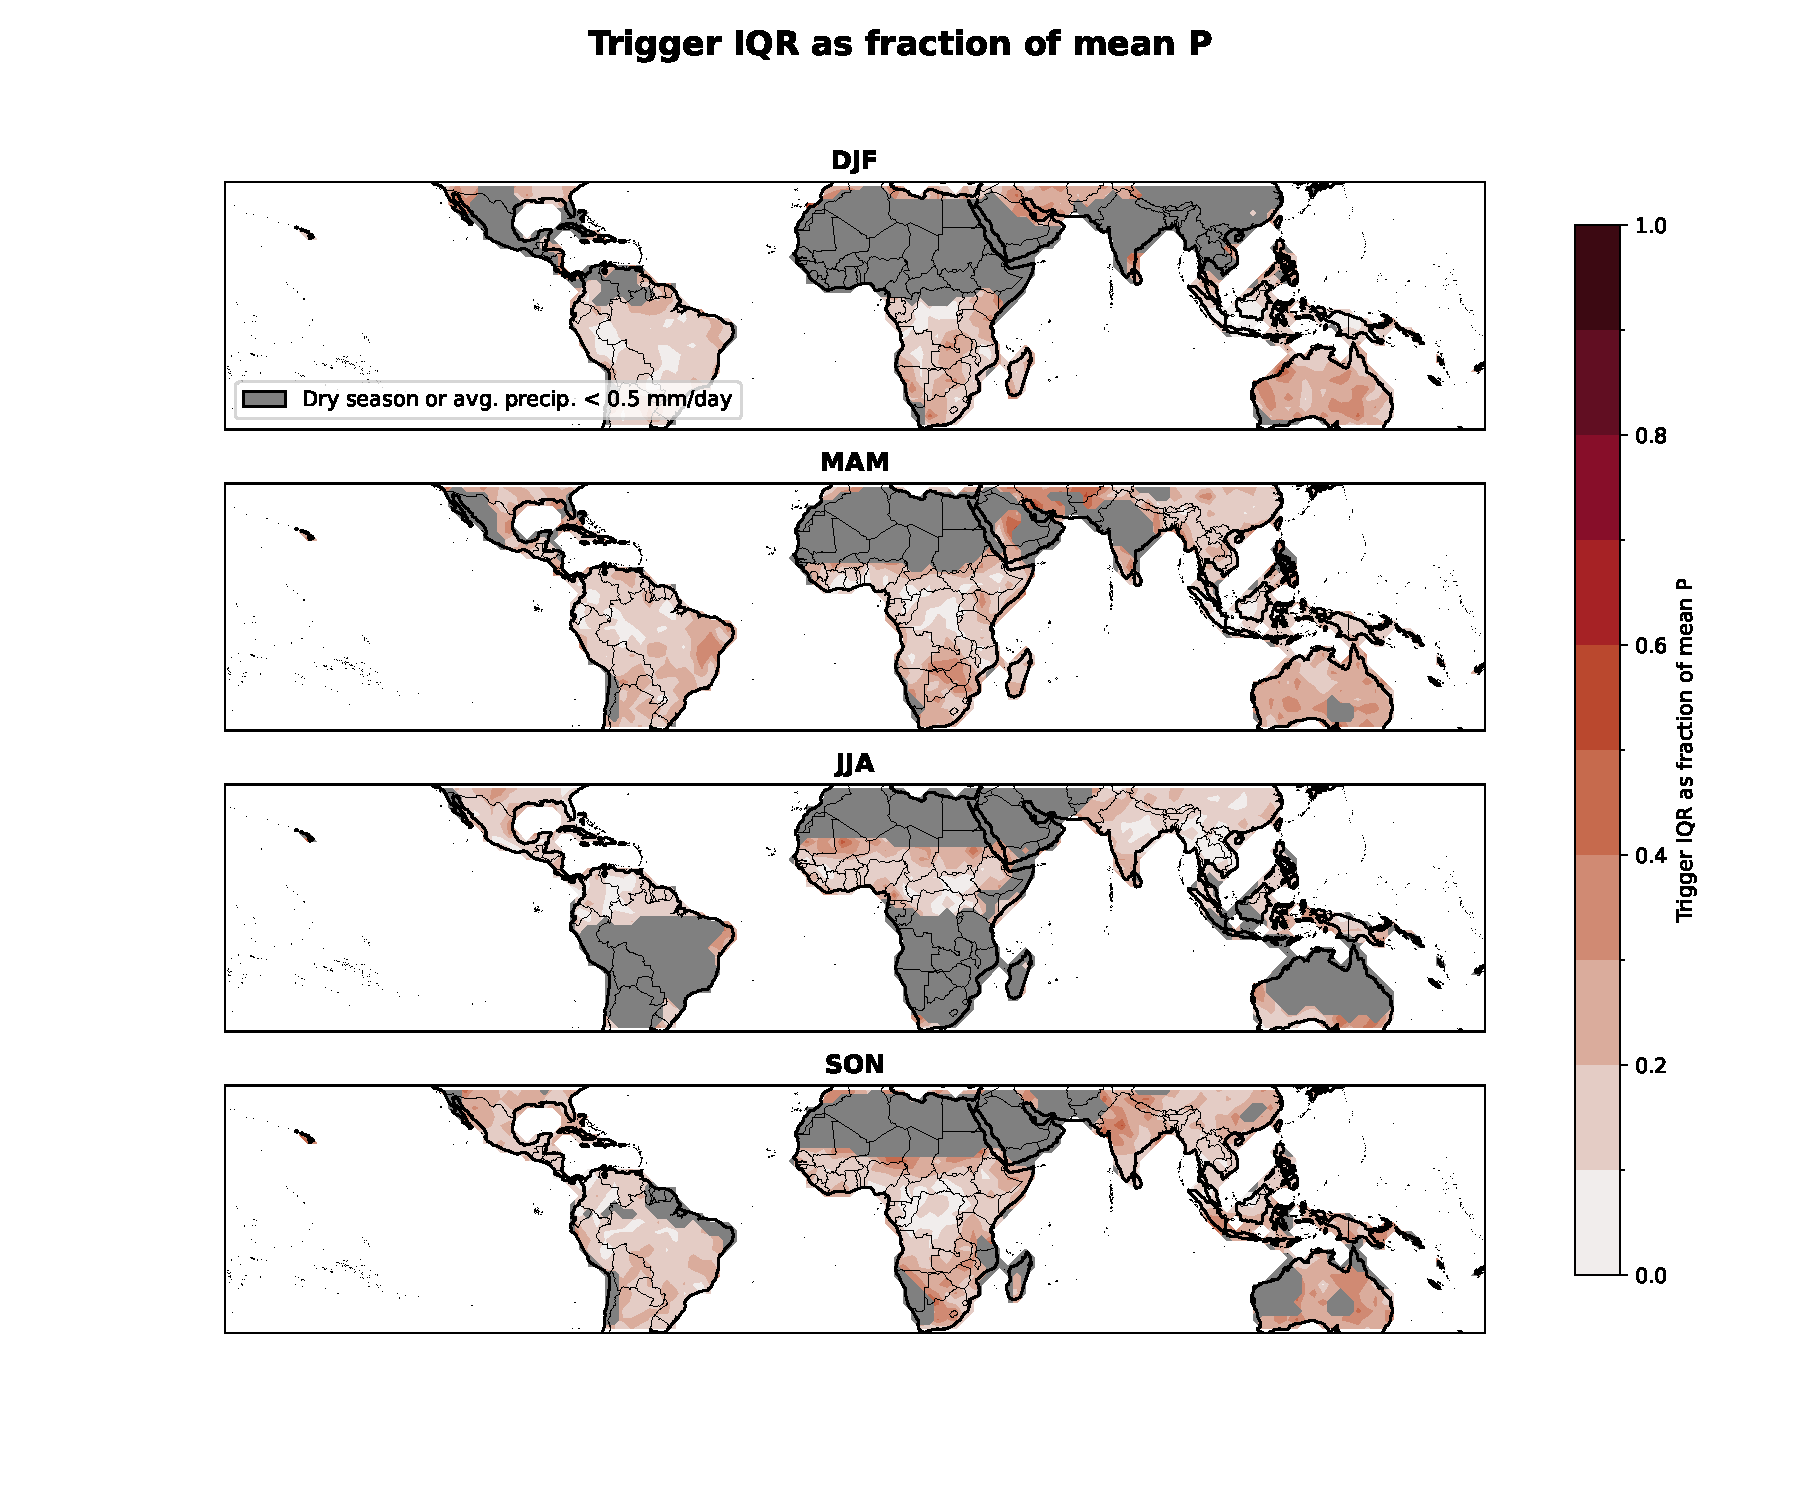
\includegraphics[width=30pc,angle=0]{2. figures/GPCP_maps.pdf}\\
\appendcaption{A1}{Summary of bootstrapped variability in GCPC seasonal rainfall extremes, summarized as the IQR of bootstrapped 20th percentile estimates divided by the mean precipitation in that pixel. Dry season areas (defined as TK) shaded in grey.}
\end{figure}

\textbf{Figure 2} illustrates the same method applied to hindcast data from CFS instead of observed rainfall. The CFS model is among those commonly used by WFP for downscaled seasonal forecasting.

\section{Application to WFP assistance programs}

Finally, we illustrate how the results of our bootstrapping method could be applied to a common problem in forecast-based humanitarian decision-making. We focus on the case of the Somali region of Ethiopia, which is highly sensitive to drought. GCMs have known limitations in modeling the agriculturally March-April-May rains in this region \citep{schwarzwald_large-scale_2023}; as such, WFP is often faced with forecasts of drought in this region that are uncertain or ambiguous due to low calibrated model confidence. This leads to situations in which local decision-makers must exercise discretion in whether or not to trigger action on the basis of a borderline drought forecast, as detailed in \textbf{Section 2c}. 

The 2021 MAM season drought is a prime example of this issue - while many indicators on the ground pointed toward heightened risk of drought impact, GCM-based forecast methods failed to predict the full extent of this drought, leading to costly inaction \citep{funk_tailored_2023}. While in hindsight, the 2021 MAM season was a clear case in which the use of local expert discretion could have adverted a costly mistake, discretion cannot be exercised on a completely ad hoc basis if anticipatory action is to remain predictable, transparent and financially sustainable. Decision-makers need a way of quantifying the range of situations in which they might reasonably exercise discretion given an ambiguous seasonal outlook.  

Our bootstrapping method offers a practical solution to this problem. To illustrate how it might be applied, \textbf{Figure 3} depicts the cumulative distribution of MAM hindcasts from the CFS model (the black slope). The empirical trigger threshold - here, the 20th percentile - is shown by the dotted red vertical line. The CDF of bootstrapped replicates of the trigger threshold is shown by the blue slope. This figure tells us that based on bootstrapped resampling, the plausible range of trigger values (the 25th-75th percentile range) falls between XX millimeters above or below the empirical value of YY.  

If the current forecast is outside of this sensitivity range, this indicates to the decision-maker that there is statistically robust evidence that the forecasted conditions are above or below the threshold. If the current forecast falls within the sensitivity range, this indicates that the decision-maker should interpret the trigger result for the current season with caution, as the appearance of trigger (un-)worthy conditions could be occurring just by chance. We can see that the 2021 season forecast (the green dot on \textbf{Figure 3}) was such a case, falling just ZZ millimeters below the trigger threshold. In this case, decision-makers faced with an uncertain outlook would have been \textit{ex ante} justified in exercising discretion in whether or not to trigger, as based on our statistical analysis. Since regional vegetation conditions leading into the MAM 2021 season were below average, and the previous OND season was poor, this was a case in which exercising heightened caution in the trigger decision would have been appropriate \citep{mauerman_long-term_2023}. 

\section{Conclusions and best practices}

% Max to draft and Dan to refine.

Uncertainty due to the limited historical record of extreme events is a significant issue for forecast-based anticipatory action, but is rarely accounted for when quantifying uncertainty. Our methodology proposed in this paper offers a solution to this problem that can be implemented easily (example Python code is provided in the Supplementary Material), requires minimal assumptions, and is robust to interannual and decadal correlation in the historical record. The method is agnostic to the type of data used, and could accommodate more elaborate forecast-based decision rules so long as the historical data necessary to evaluate those rules is available. Examining United Nations operational AA forecasts in sub-Saharan Africa, we demonstrate how our method provides a better quantification of critical underlying uncertainty, enabling these AA systems to meet the state-of-the-art demanded by donors and the WMO.


%%%%%%%%%%%%%%%%%%%%%%%%%%%%%%%%%%%%%%%%%%%%%%%%%%%%%%%%%%%%%%%%%%%%%
% ACKNOWLEDGMENTS
%%%%%%%%%%%%%%%%%%%%%%%%%%%%%%%%%%%%%%%%%%%%%%%%%%%%%%%%%%%%%%%%%%%%%
\acknowledgments
Keep acknowledgments (note correct spelling: no ``e'' between the ``g'' and
``m'') as brief as possible. In general, acknowledge only direct help in
writing or research. Financial support (e.g., grant numbers) for the work
done, for an author, or for the laboratory where the work was performed is
best acknowledged here rather than as footnotes to the title or to an
author's name. Contribution numbers (if the work has been published by the
author's institution or organization) should be included as footnotes on the title page,
not in the acknowledgments.

%%%%%%%%%%%%%%%%%%%%%%%%%%%%%%%%%%%%%%%%%%%%%%%%%%%%%%%%%%%%%%%%%%%%%
% DATA AVAILABILITY STATEMENT
%%%%%%%%%%%%%%%%%%%%%%%%%%%%%%%%%%%%%%%%%%%%%%%%%%%%%%%%%%%%%%%%%%%%%
% 
%
\datastatement
The data availability statement is where authors should describe how the data underlying 
the findings within the article can be accessed and reused. Authors should attempt to 
provide unrestricted access to all data and materials underlying reported findings. 
If data access is restricted, authors must mention this in the statement.

%%%%%%%%%%%%%%%%%%%%%%%%%%%%%%%%%%%%%%%%%%%%%%%%%%%%%%%%%%%%%%%%%%%%%
% APPENDIXES
%%%%%%%%%%%%%%%%%%%%%%%%%%%%%%%%%%%%%%%%%%%%%%%%%%%%%%%%%%%%%%%%%%%%%
%
% Use \appendix if there is only one appendix.
%\appendix

% Use \appendix[A], \appendix[B], if you have multiple appendixes.
%\appendix[A]

%% Appendix title is necessary! For appendix title:
%\appendixtitle{}

%%% Appendix section numbering (note, skip \section and begin with \subsection)
% \subsection{First primary heading}

% \subsubsection{First secondary heading}

% \paragraph{First tertiary heading}

%% Important!
%\appendcaption{<appendix letter and number>}{<caption>} 
%must be used for figures and tables in appendixes, e.g.,
%
%\begin{figure}
%\noindent\includegraphics[width=19pc,angle=0]{figure01.pdf}\\
%\appendcaption{A1}{Caption here.}
%\end{figure}
%
% All appendix figures/tables should be placed in order AFTER the main figures/tables, i.e., tables, appendix tables, figures, appendix figures.
%
%%%%%%%%%%%%%%%%%%%%%%%%%%%%%%%%%%%%%%%%%%%%%%%%%%%%%%%%%%%%%%%%%%%%%
% REFERENCES
%%%%%%%%%%%%%%%%%%%%%%%%%%%%%%%%%%%%%%%%%%%%%%%%%%%%%%%%%%%%%%%%%%%%%
% Make your BibTeX bibliography by using these commands:
% \bibliographystyle{ametsoc2014}
% \bibliography{references}

\bibliographystyle{ametsoc2014}
\bibliography{references}

%%%%%%%%%%%%%%%%%%%%%%%%%%%%%%%%%%%%%%%%%%%%%%%%%%%%%%%%%%%%%%%%%%%%%
% TABLES
%%%%%%%%%%%%%%%%%%%%%%%%%%%%%%%%%%%%%%%%%%%%%%%%%%%%%%%%%%%%%%%%%%%%%
%% Enter tables at the end of the document, before figures.
%%
%
%\begin{table}[t]
%\caption{This is a sample table caption and table layout.  Enter as many tables as
%  necessary at the end of your manuscript. Table from Lorenz (1963).}\label{t1}
%\begin{center}
%\begin{tabular}{ccccrrcrc}
%\hline\hline
%$N$ & $X$ & $Y$ & $Z$\\
%\hline
% 0000 & 0000 & 0010 & 0000 \\
% 0005 & 0004 & 0012 & 0000 \\
% 0010 & 0009 & 0020 & 0000 \\
% 0015 & 0016 & 0036 & 0002 \\
% 0020 & 0030 & 0066 & 0007 \\
% 0025 & 0054 & 0115 & 0024 \\
%\hline
%\end{tabular}
%\end{center}
%\end{table}

%%%%%%%%%%%%%%%%%%%%%%%%%%%%%%%%%%%%%%%%%%%%%%%%%%%%%%%%%%%%%%%%%%%%%
% FIGURES
%%%%%%%%%%%%%%%%%%%%%%%%%%%%%%%%%%%%%%%%%%%%%%%%%%%%%%%%%%%%%%%%%%%%%
%% Enter figures at the end of the document, after tables.
%%
%
%\begin{figure}[t]
%  \noindent\includegraphics[width=19pc,angle=0]{figure01.pdf}\\
%  \caption{Enter the caption for your figure here.  Repeat as
%  necessary for each of your figures. Figure from \protect\cite{Knutti2008}.}\label{f1}
%\end{figure}

\end{document}